\section*{CHAPTER 4: SIMULATION AND RESULTS}
\addcontentsline{toc}{section}{\numberline{}CHAPTER 4: SIMULATION AND RESULTS}
\setcounter{section}{4}
\setcounter{subsection}{0}
\setcounter{figure}{0}
\setcounter{table}{0}

In this project, we're using a python script to simulate the 64 QAM OFDM system. A 3 channels bitmap image is used as source input. Another bitmap iamge file will be generated at the end of the simulation as the output.

\subsection{Configurations and Parameters set up}

\begin{enumerate}
    \item $K = 64$ : The number of subcarriers, describes how many subcarriers are available in the OFDM system.
    \item $CP = K//$4 : The length of the cyclic prefix (CP) denotes the number of samples that are copied from the end of the modulated block to the beginning, to yield a cyclic extension of the block.
    \item $P = 8$ : The number of pilots in the OFDM symbol, describes how many carriers are used to transmit known information (i.e. pilots). Pilots will be used at the receiver to estimate the wireless channel between transmitter and receiver.
    \item $pilotValue = 3+3j$ : The known value each pilot transmits
\end{enumerate}

After that, we need to define some index sets that describe which carriers transmit pilots and which carriers contain payload.

\begin{figure}[htbp]
    \centering
     \begin{subfigure}[t]{.49\linewidth}
        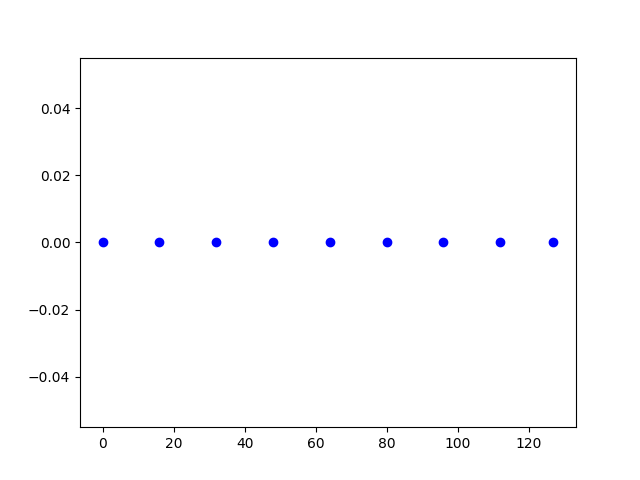
\includegraphics[width=\linewidth]{../Source/results/pilotCarriers.png}
        \caption{Pilot Carriers}
        \label{pilotCarriers}
    \end{subfigure}
    % \hfil
    \begin{subfigure}[t]{0.49\linewidth}
        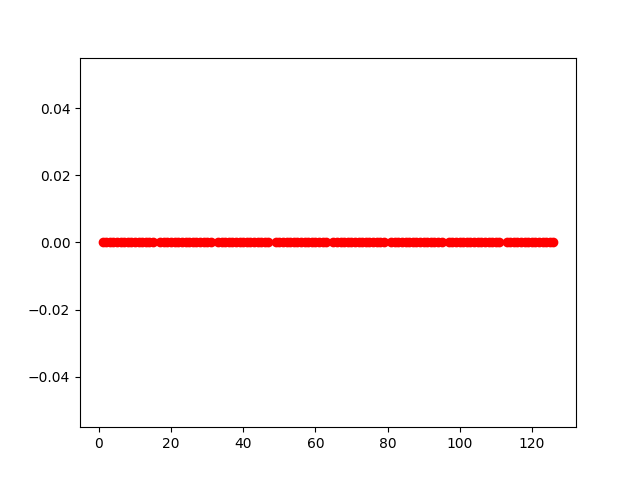
\includegraphics[width=\linewidth]{../Source/results/dataCarriers.png}
        \caption{Data Carriers}
        \label{dataCarriers}
    \end{subfigure}
    \caption{The Carriers transmit pilots and which carriers contain payload}
\end{figure}

Let's define the modulation index $\mu$ and the corresponding mapping table. We consider 64QAM transmission, i.e. we have $\mu=6$ bits per symbol. Furthermore, the mapping from groups of 6 bits to a 64QAM constellation symbol shall be defined in mapping table.

\begin{figure}[ht]
    \centering
    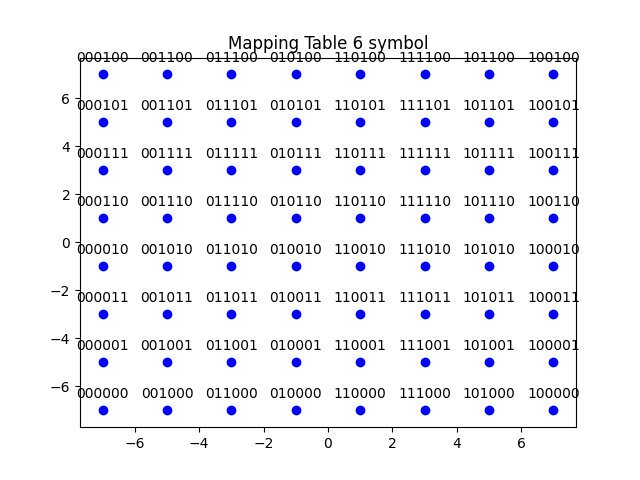
\includegraphics[width=\textwidth]{../Source/results/mapping.png}
    \caption{\bfseries\centering\fontsize{13pt}{0pt}\selectfont 64-QAM Constellation with gray-mapping}
    \label{mapping}
\end{figure}

In Figure \ref{mapping}, we have plotted the 64-QAM constellation, along with the bit-labels.
Int Gray-mapping, two adjacent constellation symbols differ only by one bit and the other 5 bits remain the same. This technique helps to minimize bit-errors, in case a wrong constellation symbol is detected: Most probably, symbol errors are "off-by-one" errors, i.e. a symbol next to the correct symbol is detected. Then, only a single bit-error occurs.

\subsection{OFDM Transmitter}

As mention earlier, the input is a 3 channels, 256x256 bitmap image (Figure \ref{input})

\begin{figure}[htbp]
    \centering
    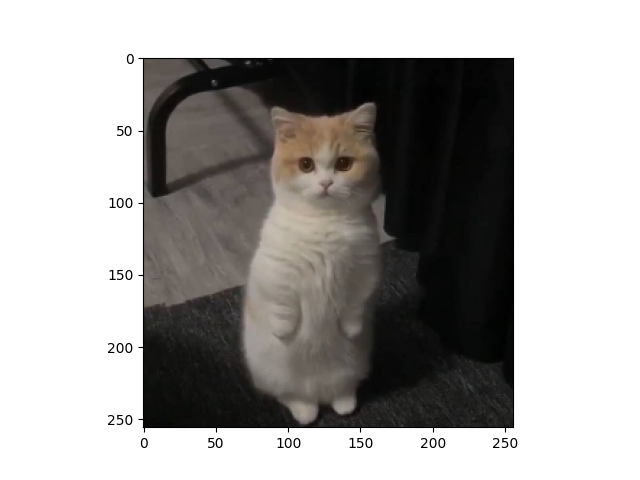
\includegraphics[width=\textwidth]{../Source/results/input.png}
    \caption{Input image}
    \label{input}
\end{figure}

\subsection{OFDM Receiver}

\begin{figure}[htbp]
    \centering
     \begin{subfigure}[t]{.49\linewidth}
        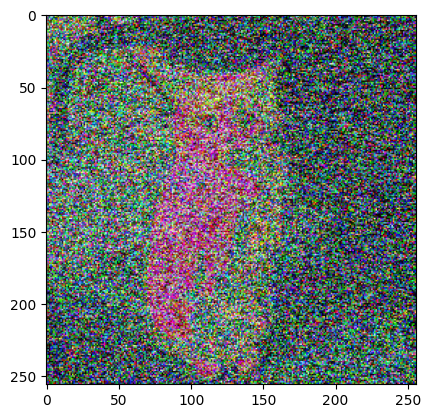
\includegraphics[width=\linewidth]{../Source/results/output_0db.png}
        \caption{SNR = 0db}
        \label{0db}
    \end{subfigure}
    \hfil
    \begin{subfigure}[t]{0.49\linewidth}
        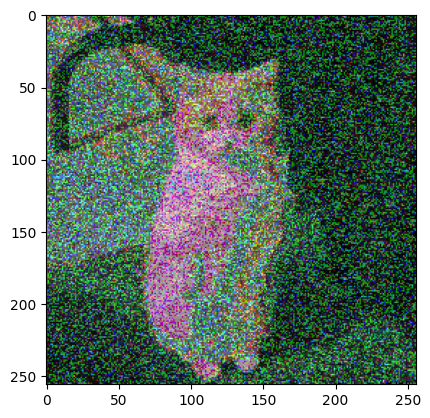
\includegraphics[width=\linewidth]{../Source/results/output_10db.png}
        \caption{SNR = 10db}
        \label{10db}
    \end{subfigure}
    \hfil
    \begin{subfigure}[t]{0.49\linewidth}
        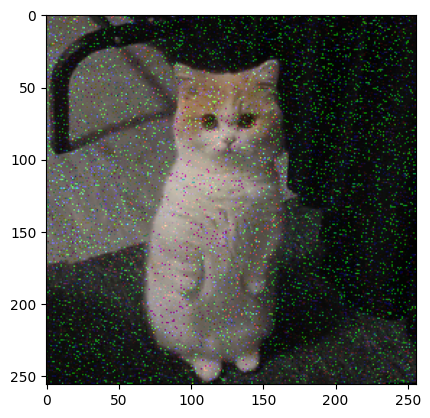
\includegraphics[width=\linewidth]{../Source/results/output_20db.png}
        \caption{SNR = 20db}
        \label{20db}
    \end{subfigure}
    \hfil
    \begin{subfigure}[t]{0.49\linewidth}
        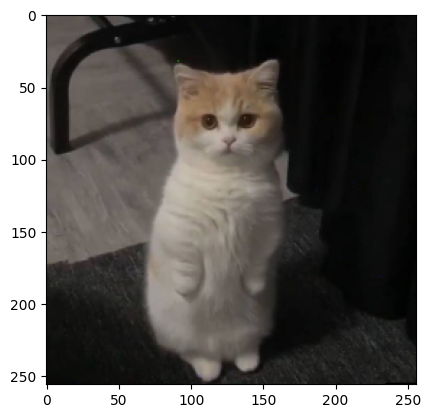
\includegraphics[width=\linewidth]{../Source/results/output_30db.png}
        \caption{SNR = 30db}
        \label{30db}
    \end{subfigure}
    \caption{The received using 64 QAM module}
\end{figure}

\begin{figure}[htbp]
    \centering
    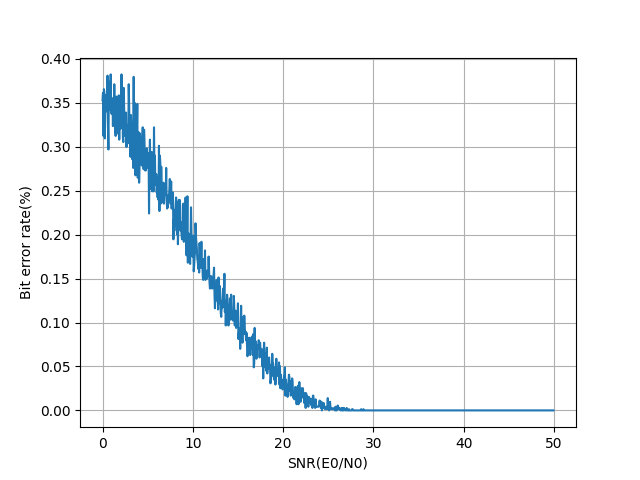
\includegraphics[width=\linewidth]{../Source/results/ber.png}
    \caption*{Plot of BER for SNRdb values from 0 to 50}
    \label{ber}
\end{figure}